\section{Grupo UFRJ e o framework Fence}
A construção do acelerador \emph{LHC} e respectivos detectores envolveu centenas de institutos ao redor do mundo, constituindo um importante trabalho cooperativo. Com o crescimento desta cooperação, diversos desafios passaram a existir a fim de garantir a qualidade da pesquisa científica produzida. O longo período de tempo levado para construção, teste e aprimoramento dos detectores e aceleradores ocasionou o armazenamento de informações utilizando diferentes tecnologias, métodos e terminologias. Acrescentando isso à descentralização de dados com a participação global de pesquisadores, fez com que a recuperação e compartilhamento de dados se tornasse gradativamente mais difícil com o tempo. Cada solução implementada atendia apenas necessidades específicas do próprio grupo na maior parte dos casos, dificultando a recuperação de dados heterogêneos e a integração de tais fontes de informação. \cite{grael}.

No contexto da colaboração entre UFRJ e \emph{ATLAS}, em 2003 um grupo de brasileiros propuseram um modelo para recuperar dados armazenados em repositórios independentemente de tecnologia, modelagem ou terminologia. Nomeado \emph{Glance}, esse modelo tinha como objetivo proporcionar uma ferramenta amigável para o próprio usuário poder customizar as suas interfaces de busca e inserção de dados \cite{maidantchik}. Esta ferramenta abstraía a complexidade do armazenamento de dados, tornando mais fácil para o usuário conseguir procurar e modificar a informação desejada. O paradigma \emph{procedural} foi adotado na arquitetura desta ferramenta, que foi escrita nas linguagens \emph{C++}, \emph{php} e \emph{Javascript}. Na época, 21 sistemas foram implementados a partir dele, atendendo além do próprio \emph{ATLAS}, os experimentos \emph{LHCb} e \emph{ALICE}.

Com a expansão do uso do \emph{Glance} pela crescente demanda de sistemas, novas oportunidades passaram a existir para os desenvolvedores \cite{ramos}. O modelo de administração empregado no \emph{CERN} e seus experimentos se baseia em uma alta rotatividade nos cargos gerenciais, e somando-se isso com os constantes avanços tecnológicos dos experimentos, a alteração de funcionalidades nos sistemas \emph{Glance} passou a se tornar algo frequente e requisitado. Uma nova administração pode ter uma expectativa distinta da anterior, assim como novos usuários podem necessitar novas soluções para atender demandas tecnológicas mais recentes.

Outra oportunidade observada foi a possibilidade de melhorar o compartilhamento de código entre os sistemas. Uma proposta como a adoção do paradigma de orientação a objetos e utilização de classes bases abstratas, contendo a funcionalidade comum, poderia reduzir a base de código total dos sistemas e facilitar a manutenção.

Tendo em vista a frequente mudança de requisitos pelos representantes da base de usuários e a evolução das tecnologias web, em 2014 foi proposto e implementado pela UFRJ o \emph{framework} \emph{Frontend Engine for Glance}, ou simplesmente \emph{Fence} \cite{lange}. O \emph{Fence} tem como objetivo reunir um conjunto de classes e ferramentas para implementar e reutilizar as interfaces entre os sistemas. Sua proposta inicial era projetar uma camada entre a recuperação dos dados provenientes do \emph{Glance} e a visualização destas informações, indo de acordo com uma série de regras estabelecidas por cada experimento. Escrito em \emph{php} e fazendo uso extensivo de herança e polimorfismo com a orientação a objetos, o comportamento das interfaces geradas pelo \emph{framework} é condicionado a arquivos de configuração \emph{JSON}. Estes arquivos funcionam como agentes de controle, podendo especificar as regras de inserção de um formulário ou os critérios disponíveis de busca. Esta abordagem permite que os sistemas possam ser projetados ou adaptados às variações de seus requisitos com menor necessidade de escrita de código.

Atualmente existem 27 sistemas e subsistemas em web que foram desenvolvidos a partir do \emph{framework} \emph{Fence} \cite{fence}. Tais sistemas são responsáveis por apoiar os principais aspectos da colaboração, como os membros dos experimentos, contratos, institutos, publicações, equipamentos e configurações dos detectores. Na figura \ref{fig:aces-websystem}, o sistema \emph{ACES} para administração de equipamentos, criado a partir do \emph{framework} \emph{Fence}.

\begin{figure}[H]
    \centering
    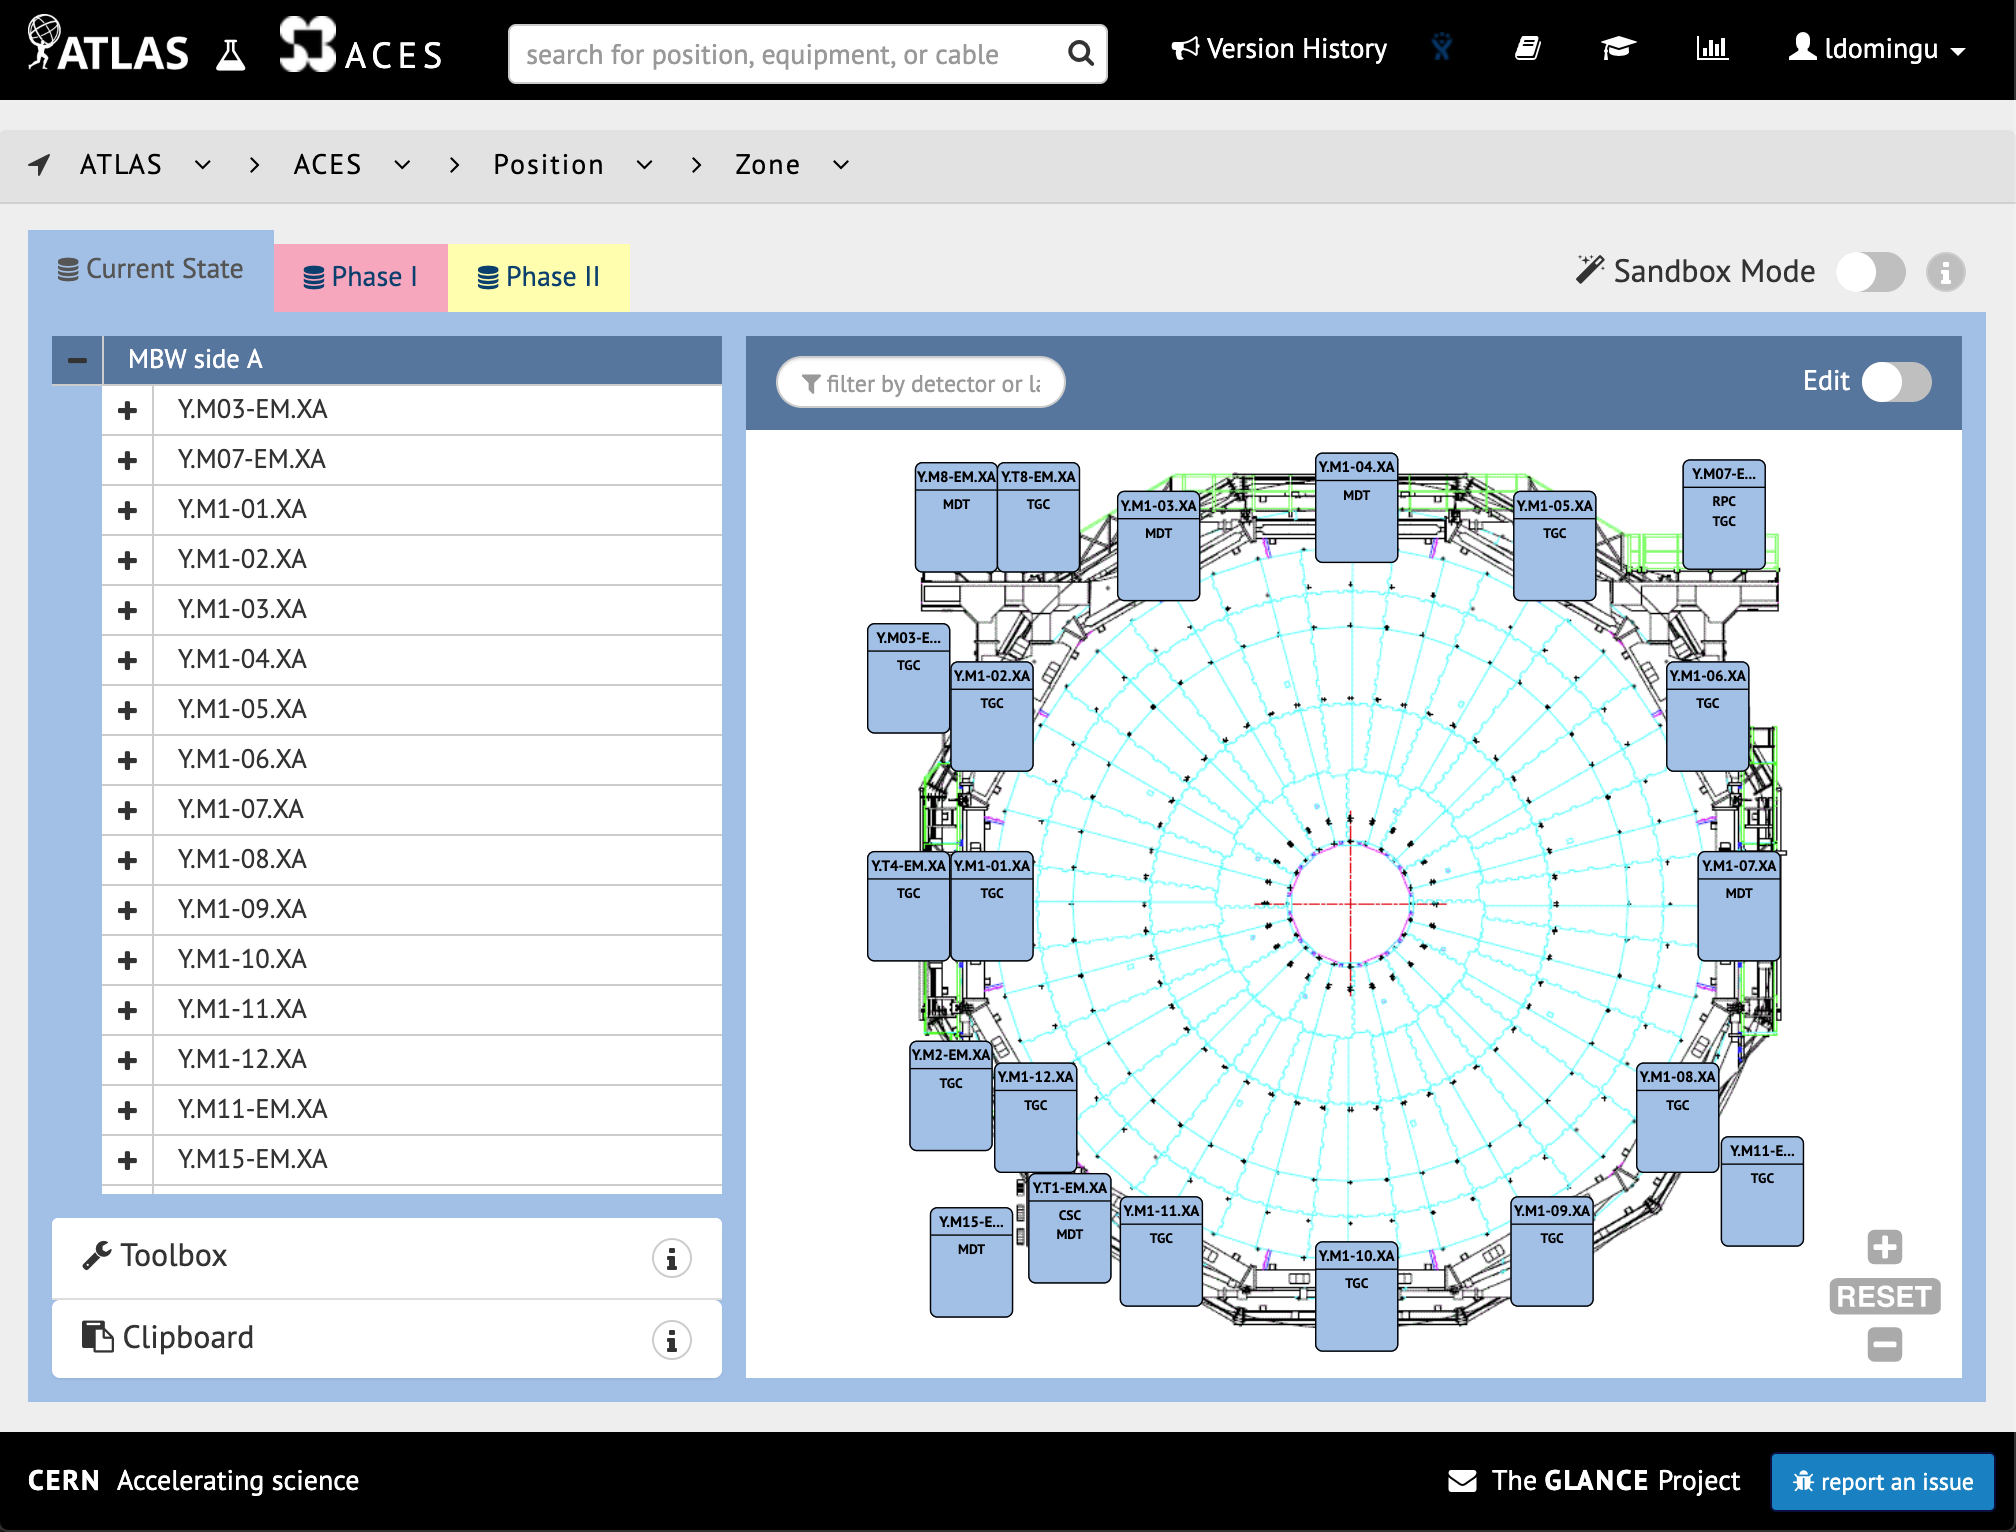
\includegraphics[width=15cm]{source/2-contextualizacao/images/aces-websystem.png}
    \caption{Captura de tela do sistema \emph{ACES}, responsável por gerenciamento de equipamentos.}
    \label{fig:aces-websystem}
\end{figure}
